\newpage
\section{Ogólne określenie wymagań}		%1
%Określenie celu pracy, co chcemy uzyskać, jakie przewidujemy wyniki

Celem niniejszego projektu jest zaimplementowanie i przetestowanie struktury danych typu dwukierunkowa lista wiązana w języku C++. Oczekiwanym wynikiem jest stworzenie efektywnego kontenera dynamicznego, który umożliwia operacje wstawiania, usuwania oraz przeglądania elementów zarówno w kierunku rosnącym, jak i malejącym. Program ma na celu zaprezentowanie poprawnego zarządzania pamięcią dynamiczną oraz operacji na wskaźnikach.

\subsection{Struktura i implementacja listy}  %1.1       

Każdy element listy dwukierunkowej jest reprezentowany przez osobny węzeł. Jeśli chcemy odwołać się do literatury naukowej lub dokumentacji, wykonujemy to w~ten sposób.

%rysunek
\begin{figure}[!htb]
	\begin{center}
		
\includegraphics[width=0.8\linewidth]{rys/lista.drawio.png}
		\caption{Schemat powiązań w liście dwukierunkowej}
		\label{rys:rysunek001}
	\end{center}
\end{figure}

Węzeł przechowuje wartość całkowitą oraz dwa wskaźniki: na poprzedni oraz następny element.\\Węzeł początkowy posiada wskaźnik poprzednika ustawiony na wartość pustą (`nullptr`). 
Rysunek \ref{rys:rysunek001} (s. \pageref{rys:rysunek001}) pokazuje schemat powiązań między węzłami listy.

%tabelka
\begin{tabela}
	{Złożoność obliczeniowa operacji}	%opis w spisie tabel
	{Złożoność obliczeniowa operacji}	%opis przy tabeli
	{
		\begin{tabular}{|c|c|c|} \hline
			Operacja & Złożoność czasowa & Złożoność pamięciowa \\ \hline
			Dodanie na początek/koniec & $O(1)$ & $O(1)$ \\ \hline
			Wyszukanie elementu & $O(n)$ & $O(1)$ \\ \hline
			Usunięcie elementu & $O(n)$ lub $O(1)$ & $O(1)$ \\ \hline
		\end{tabular}
	}
	\label{tab:tablica001}
\end{tabela}

Tabela \ref{tab:tablica001} (s. \pageref{tab:tablica001}) przedstawia zestawienie złożoności obliczeniowej dla podstawowych operacji na liście dwukierunkowej.

% Kod
\subsection{Kod źródłowy węzła}

Kod \ref{lst:listing-cpp} (s. \pageref{lst:listing-cpp}) przedstawia implementację klasy pojedynczego węzła, która stanowi fundamentalny budulec struktury listy dwukierunkowej.

\begin{lstlisting}[caption=Definicja struktury węzła Node, label={lst:listing-cpp}, language=C++]
#ifndef NODE_H
#define NODE_H

class Node {
public:
    int data;     // Wartosc przechowywana w wezle
    Node* prev;   // Wskaznik na poprzedni wezel
    Node* next;   // Wskaznik na nastepny wezel

    // Konstruktor inicjalizujacy wezel
    Node(int val) : data(val), prev(nullptr), next(nullptr) {}
};

#endif
\end{lstlisting}

\subsection{Zarządzanie pamięcią i testowanie}  %1.2

Ponieważ lista dwukierunkowa alokuje pamięć dynamicznie przy każdym dodaniu nowego elementu za pomocą operatora `new`, kluczowym elementem projektu jest poprawnie napisany destruktor oraz metoda czyszcząca.

Każde usunięcie elementu wymaga odpowiedniego przepięcia wskaźników `prev` oraz `next` sąsiadujących węzłów, a także zwolnienia pamięci operatorem `delete`. Zapobiega to groźnym wyciekom pamięci (ang. \textit{memory leaks}). Testowanie poprawności implementacji odbywa się poprzez sekwencję operacji w pliku głównym programu (`main.cpp`), gdzie sprawdzane są skrajne przypadki, takie jak operacje na pustej liście czy usuwanie jedynego elementu.

%rysunek
\begin{figure}[!hbt]
	\begin{center}
		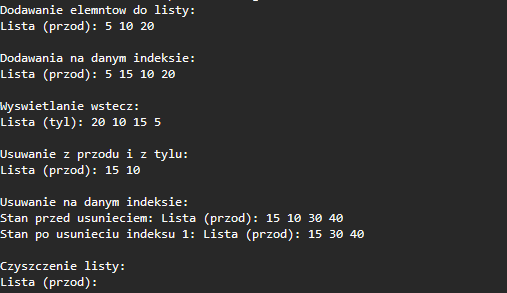
\includegraphics[width=0.9\linewidth]{rys/test1.png}
		\caption{Wynik działania testów listy (operacje wyświetlania, dodawania, usuwania)}
		\label{rys:testy_dzialania}
	\end{center}
\end{figure}

Następnym krokiem w procesie rozwoju oprogramowania jest kontrola wersji z użyciem systemu Git. Na rysunku \ref{rys:testy_dzialania} (s. \pageref{rys:testy_dzialania}) zaprezentowano przykładowy widok pomyślnego przejścia testów.